\section{Runtime Application Tuning} \label{rat}

Once the DTA analysis is finished and the ATM has been generated, the application can be used in production. 

The Runtime Application Tuning (RAT) phase of READEX is carried out by the low-overhead READEX Runtime Library (RRL). 

The RRL is implemeted as a Score-P Substrate Plugin using the Substrate Plugin Interface \cite{Schoene2017}. This plugin interface allows to utilize the instrumentation infrastructure of Score-P, without direct integration into Score-P. This approach acts to reduce maintenance and integration efforts by keeping the RRL as a separate entity. As a substrate plugin, the RRL receives notifications for differents events occuring during the application run through various means of instrumentation and uses this information to make switching decisions based on the application tuning model created at design time.

At runtime, the RRL obtains the set of configurations, in the form of scenarios, classifiers and selectors, from the ATM generated by PTF at design-time.

The RRL implements three main mechanisms in order to apply the dynamic configuration switching at runtime, namely, scenario detection, configuration switching and calibration. The following sections detail the first two mechanisms, while Section~\ref{sec:calibration} describes the calibration mechanism, which is an extension to the standard version. Figure~\ref{fig:rrl} shows the detailed architecture of RRL, and will be used to explain the three mechanisms mentioned above. 

%\begin{figure}[!t]
%\centering
%%\includegraphics[trim={7cm 2cm 5.5cm 2cm},clip,width=3in]{readex-approach}
%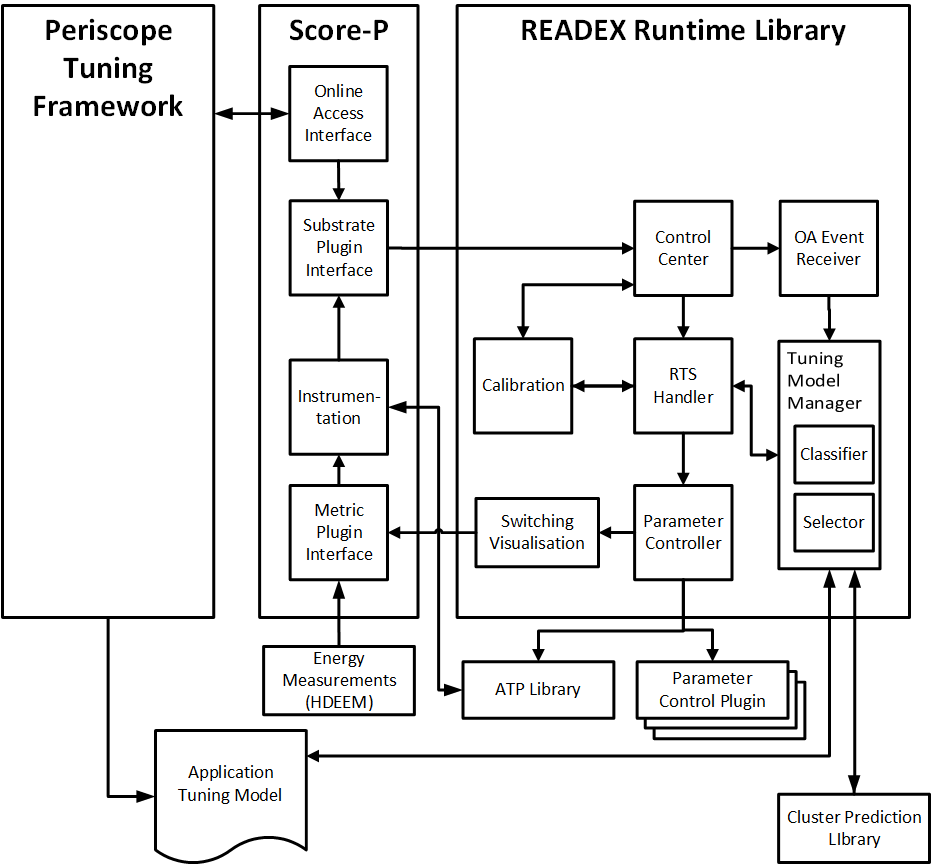
\includegraphics[width=.8\columnwidth]{figures/RRL_Architecture.png}
%\caption{Architecture of the READEX Runtime Library (RRL)}
%\label{fig:rrl}
%\end{figure}

\subsection{Scenario Detection}\label{scenario-detection}
 Runtime detection of the upcoming scenario is a process that involves several modules in the RRL architecture depicted in Figure~\ref{fig:rrl}. A production run of an application starts with a loading of the ATM into the Tuning Model Manager (TMM). When a new region is entered during the application execution, the Control Center receives notification from Score-P. The Control Center passes this information to the RTS handler, which asks if the region encountered is significant from TMM. If the TMM can find the region in ATM, then it is a significant region otherwise it is marked as an unknown region. The RTS Handler next checks the granularity of the current region. If the granularity of the region is above 100ms, only then the region is tuned. If the region is significant and has granularity above threshold, the RTS Handler first requests for the number of additional identifiers from the TMM. Once the required number of additional identifiers are collected by RTS Handler through \textit{user parameter} event notifications, the current rts is identified by both the call stack (maintained in the RTS Handler) and the additional identifiers.
RTS Handler then requests a new configuration for the current rts from the TMM which is then passed to the Parameter Controller by RTS handler to apply the configuration switching.  
If it is an unknown region and the granularity is above the threshold of 100ms, then the calibration mechanism is invoked.

\subsection{Configuration Switching}\label{config-switching}
 Switching of parameter settings is performed through the parameter control plugins that are also employed during the DTA phase.
During scenario detection, if the region entered is found to be significant by the RTS Handler and has high enough granualrity, the RTS Handler gets a new configuration from the TMM for the current rts. 
This configuration is passed to the Parameter Controller, which sets the configuration through the respective Parameter Control Plugins (PCP).

Before the current region exits, the RTS Handler receives the notification  from Score-P through Control Center. 
The RTS Hander checks if the current region was set up for calibration. If yes, it requests the configuration for the currently exited region from the
Calibration module. Once the RTS handler gets back the configuration from the calibration module, it passes this configuration to the TMM which stores the new configuration for the respective rts. If the region was not set up for calibration, then the Parameter Controller is informed that it might want to unset the current configuration. 

The Parameter Controller supports two different modes: \textit{reset} and \textit{no-reset}. The first mode maintains a configuration stack. Whenever a new configuration is set, the previous configuration is pushed onto this stack. When the corresponding unset occurs, the element is removed from the stack and the previous configuration is set. If the no-reset mode is selected, the current configuration stays active until a new configuration is set. The unset is ignored. This behaviour is configurable by the user. By default, \textit{reset} mode is enabled.

\subsection{Calibration}\label{calibr}
 For the already seen rts's, RRL extracts the optimal configuration from the ATM. For the un-seen ones, the RRL calibration mechanism, explained in Section~\ref{sec:calibration}, is used to find the optimal system configuration based on machine learning algorithms and the data stored in the tuning model. 

 